\documentclass[12pt]{article}
\usepackage{geometry}                % See geometry.pdf to learn the layout options. There are lots.
\geometry{letterpaper}                   % ... or a4paper or a5paper or ... 
\usepackage{graphicx}
\usepackage{amssymb}
\usepackage{amsthm}
\usepackage{epstopdf}
\usepackage[utf8]{inputenc}
\usepackage[usenames,dvipsnames]{color}
\usepackage[table]{xcolor}
\usepackage{hyperref}
\DeclareGraphicsRule{.tif}{png}{.png}{`convert #1 `dirname #1`/`basename #1 .tif`.png}

\theoremstyle{definition}
\newtheorem{example}{Example}

\newenvironment{explanation}{%
   \setlength{\parindent}{0pt}
   \itshape
   \color{blue}
}{}

\newcommand{\projectname}{PanSim}
\newcommand{\productname}{Pandemic Simulator}
\newcommand{\projectleader}{O. Dominik}
\newcommand{\documentstatus}{In process}
%\newcommand{\documentstatus}{Submitted}
%\newcommand{\documentstatus}{Released}
\newcommand{\version}{V. 1.0}

\begin{document}
\begin{titlepage}
\begin{flushright}

\includegraphics[scale=.5]{htlleondinglogo.png}\\
\end{flushright}

\vspace{10em}

\begin{center}
{\Huge Project Proposal} \\[3em]
{\LARGE \productname} \\[3em]
\end{center}

\begin{flushleft}
\begin{tabular}{|l|l|}
\hline
Project Name & \projectname \\ \hline
Project Leader & \projectleader \\ \hline
Document state & \documentstatus \\ \hline
Version & \version \\ \hline
\end{tabular}
\end{flushleft}

\end{titlepage}
\section*{Revisions}
\begin{tabular}{|l|l|l|}
\hline
\cellcolor[gray]{0.5}\textcolor{white}{Date} & \cellcolor[gray]{0.5}\textcolor{white}{Author} & \cellcolor[gray]{0.5}\textcolor{white}{Change} \\ \hline
November 03, 2011&P. Bauer/T. Stütz&First version \\ \hline
\end{tabular}
\pagebreak

\tableofcontents
\pagebreak

\section{Introduction}

Our team decided to simulate a pandemic to help contain future panedemics more swiftly.
During the current corona crisis it has become apparent that we need some way to predict the direction of a pandemic.
In terms of feasebility we would first simulate a virus with just numbers and no graphical elements but later on we will incorperate a GUI if it is necessary.
Since this is a purely scientific simulation done by students affordability and market and economic efficiency can not be determined.
Since there isn't any funding involved in this project there are no risks only opportunities.


\pagebreak

\section{Initial Situation}

The current corona crisis has shown us that an pandemic cannot be foreseen and needs to be dealt with as fast as possible in order to stop it is spread.

Currently measures like masks, shields or curfews cannot be tested unless they have shown some effect to stop the spread of a virus.

Currently, there are many diffrent simulations that try to predict the future of the corona crisis,
and only the corona crisis. 

The Austrian government provides weekly predections on the corona virus based on the current situation in austria, from sources like that its also possible to update the simulation and guarantee a more precise outcome of the data.

Those simulations are made to try to find out when the pandemic will finaly end,
so they do not offer the possability to change the properties of the virus or to add new measures to test those.
Also many of the simulations that do offer such settings are really hard to read and do not explain their graphs in enough detail.

\pagebreak

\section{General Conditions and Constraints}

Our data needs to be obtained through trustworthy sources like government websites, universities etc.
This includes data on the virus as well as how to simulate viruses.
If we arent able to do that the whole simulation will give imprecise and false results.
So it is very necessary to get our informations from officaly and trustworthy sources. 

Also we currently lack the expertise to do such simulations which means we need to do some research first.
Otherwise we only create a simulation of how we think a simulation works and not how it should really work based on real data, events, etc.

Because of our limited computing power the simualtion cant be to complex.
\pagebreak

\section{Project Objectives and System Concepts}

Our results shall be presented as clear and easy readable as possible, 
that means that data like infectionsrate, susceptible, infected, casualties and recovered should be displayed on a graph.
Were planing on a single graph with diffrent colored lines that will show differnet data like you can see on the following picture under this text.

Calculations of the virus shall reflect a real and clear scenario with as much precision as possible.

We thought that it would be the simplest way to create a table where initial data and also outcoming data which is not shown on the graph is displayed. 
Therefore all initial data for the virus, event probability, etc. must be displayed.

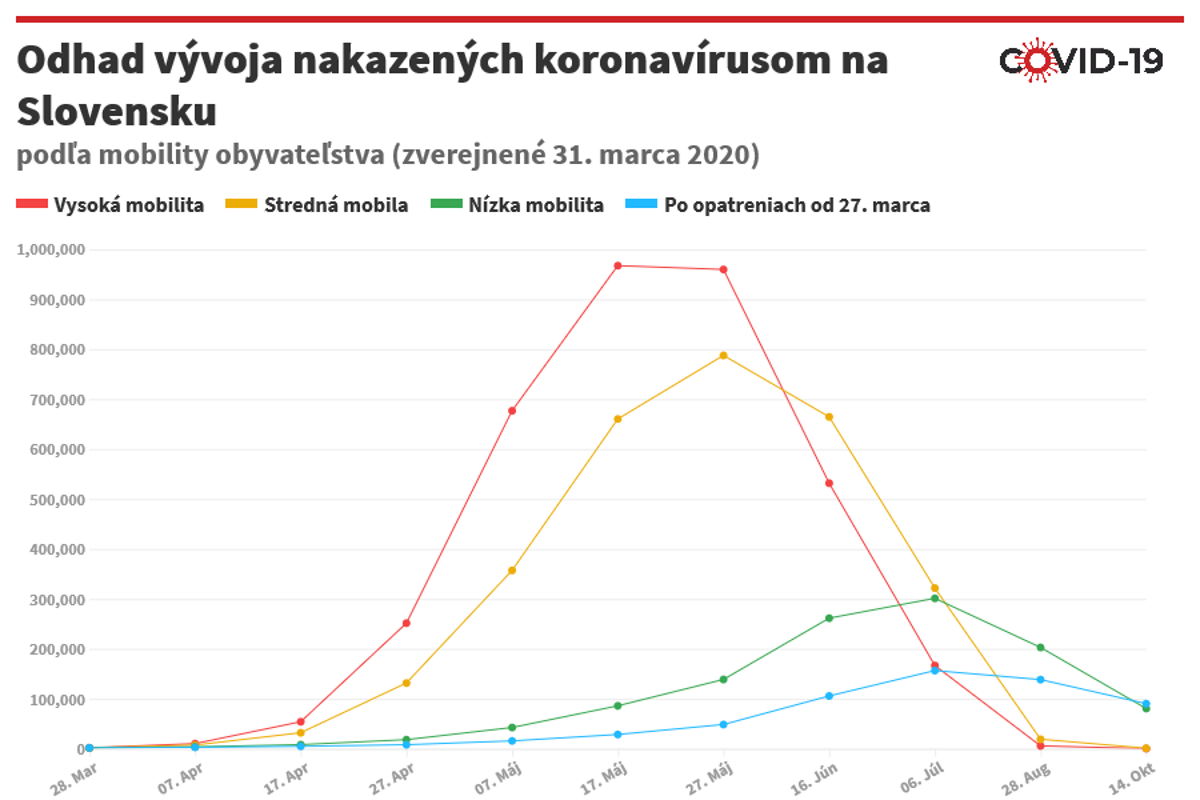
\includegraphics[width=\textwidth]{graph.png}\\
Here you can see corona graph of Slovenia in this way we want to show our calculated data. Every colored line stands for a differnet sector.

For example: blue for recovered, red for deaths and yellow for current infections.

\pagebreak
\section{Opportunities and Risks}

The first and most obvious opportunity is that we can predict current and future pandemics and therefore act swifter and more precise.
Building up from there we plan on displaying the results in a way that is easily readable for everyone so that it can be used as a proper source.

Because of the high attention this project will receive due to corona it shall be communicated very well at public events of the HTL Leonding.
The government will probably see these presentations and maybe support our project with data and/or hardware.

We currently have no idea how to simulate a virus and don't know how long it will take us to learn that knowledge

If our simulations get too complex and our laptops can't handle them anymore we have to move our calculations to a cloud or find another solution which could delay development.

\pagebreak
\section{Planning}

The first step to complete this project will be create a list of features that the simulation shall have.
We will collect all knowledge about the mathmatics of a pandemic that is necessary to implement those features and edit the list so that all the features are possible to implement in the given time.
As a Deadline for this step we will set january 14th. 

After that we will start with the actual programming.
The first simple prototype should be ready by feburary 4th. After that we will need another week to implement a graph with the results that the prototype put out.


At this point we will start adding features from our list. On May 16th our simualtion should be ready test using real life pandemics. 
We will be doing this by trying to recreate real life pandemics and compareing the simulated data with the actual data.


If there is still some time left we will use it to implement an easy to understand graphical user interface.

\end{document}  